\begin{figure}[htbp]
\centering
\caption{
An introduction to Modern Portfolio Theory mean-variance optimization.
}
\label{fig:mpt}
\end{figure}

\clearpage

\begin{figure}[htbp]
\centering
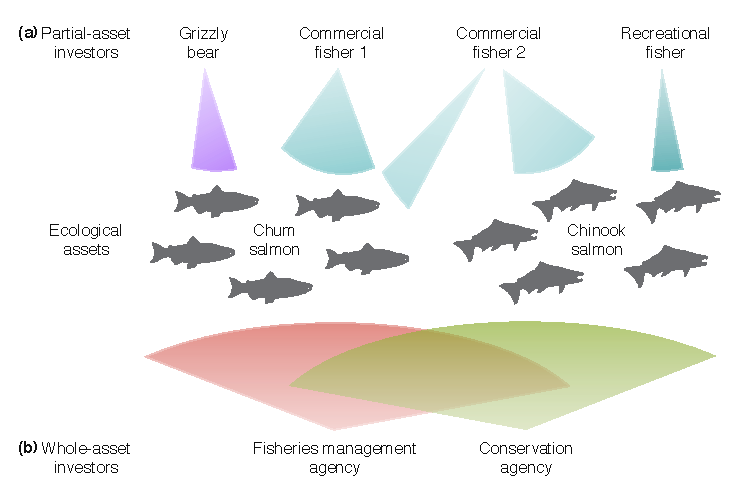
\includegraphics[width=5in]{salmon-portfolios.pdf}
\caption{
There are multiple ways of investing in ecological portfolios.
In this example, investors are shown along the top and bottom and ecological assets are shown in the middle (populations of chum salmon, \textit{Oncorhynchus keta}, and Chinook salmon, \textit{Oncorhynchus tshawytscha}).
The shaded arcs indicate investment.
\textbf{(a)} Partial-asset investors invest by removing portions of the salmon populations --- the salmon that commercial fisher 1 removes are unavailable for the grizzly bear.
These investors can often change their investment with ease.
For example, commercial fisher 2 could decide to fish more Chinook and less chum salmon.
Most financial portfolio theory is developed around this paradigm.
\textbf{(b)} Whole-asset investors invest in entire populations.
These investors can share assets but may have different goals for their portfolio.
They can adjust their investment by managing properties of the population itself.
For example, the fisheries management agency could reduce fishing of chum salmon to allow the population to grow.
The conservation agency could fund habitat restoration for Chinook salmon to increase carrying capacity and expand their investment.}
\label{fig:salmonport}
\end{figure}

\begin{figure}[htbp]
\centering
\caption{
Risk vs. variance; how they differ and what is a coherent risk metric?
A figure illustrating time series with the same variance but different risk properties.
}
\label{fig:risk}
\end{figure}
